\chapter{Biodata Penulis}

\begin{wrapfigure}{l}{4cm}
    \vspace{-20pt}
    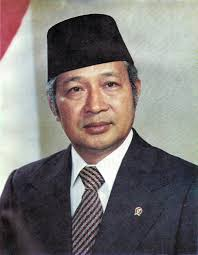
\includegraphics[width=3.95cm]{gambar/soeharto.jpeg}
    \vspace{-20pt}
\end{wrapfigure}

Ari Setiawan lahir di Sidoarjo pada 1 Agustus 1996. Pendidikan formal dimulai dari TK hingga SMA, yang seluruhnya ditempuh di Sidoarjo, dan penulis lulus dari SMA Hang Tuah 2 Sidoarjo pada tahun 2014. Setelah itu, penulis diterima di Departemen Teknik Kelautan, Fakultas Teknologi Kelautan, Institut Teknologi Sepuluh Nopember Surabaya melalui jalur SBMPTN. Selama perkuliahan, penulis aktif sebagai kepala divisi pemetaan dalam Pengembangan Sumber Daya Mahasiswa Himpunan Mahasiswa Teknik Kelautan pada periode 2016-2017. Dalam kegiatan kerja praktek di PT. Dok dan Perkapalan Surabaya, penulis mengambil studi kasus mengenai kapal KMP SMS Swakarya yang telah selesai direparasi dan siap dioperasikan. Penulis memiliki ketertarikan dalam bidang hidrodinamika, dan melalui tugas akhir ini, penulis menerapkan studi kasus di bidang tersebut. 
